\documentclass[12pt]{article}
\usepackage{graphicx}
\usepackage{amsmath}
\usepackage{cite}


\title{State-of-the-Art Review of Generative Adversarial Networks (GANs) in Medical Applications}
\author{Flesar Radu-Constantin}
\date{January 2025}

\begin{document}

\maketitle

\begin{abstract}
Generative Adversarial Networks (GANs) have emerged as a critical tool in many medical applications including image generation and reconstruction, as well as diagnostic support. Abstract Generative adversarial networks (GANs) have gained widespread attention from researchers all over the world, and in this paper, we provide a systematic review of GAN applications in medicine featuring recent advancements in high-resolution image generation, volumetric data synthesis, artefact removal, and data augmentation to apply on top machine learning based models. This paper provides insights from recent efforts to harness GANs to improve the quality and accessibility of medical imaging and data and discusses the potential role of GANs in modern healthcare.
\end{abstract}

\section{Introduction}

The rapid development of artificial intelligence (AI) has provided us with strong and novel methods to address issues in medical imaging and diagnostics. Out of these, the Generative Adversarial Networks (GANs) were first proposed by Goodfellow et al. The advent of deep learning algorithms in 2014 has proved to be a key transforming tool for synthesizing and improving medical images. GANs feature two antagonistic neural networks, creating extremely realistic representations of the data in question – a generator and a discriminator. It is this adversarial setup that allows GANs to create images and other data types that are similar to real-world objects and may have large potential in medicine.

High-quality images are essential for medical imaging and diagnostic practices, however, obtaining enough labelled medical data is expensive, time-consuming, and restricted by patient privacy concerns. Generative adversarial networks (GANs) are powerful tools that are capable of generating novel high-resolution images along with 3D volumetric data, potentially increasing the scale and diversity of data that can be provided for training diagnostic algorithms. Recent works have shown and enabled GANs to synthesize medical images, reducing noise, correcting artefacts, and making these imaging systems more reliable for diagnostics.

Generative Adversarial Networks (GANs) are being utilized in various medical fields, such as imaging of the brain, heart, and lungs, as well as in analyzing conditions like Parkinson's disease using non-imaging data. For example, GANs have been used to minimize radiation exposure in CT scans by creating high-quality images from low-dose inputs, a method discussed by Vey et al. \cite{Vey2019}. Furthermore, the research by Du and Tian \cite{Du2024} on integrating GANs with Transformers demonstrates how GANs can be improved to generate super-resolution images, which enhances diagnostic accuracy.

This paper seeks to offer a thorough review of the most recent applications of GANs in medical imaging, exploring progress in synthetic data generation, diagnostic assistance, and improvements in image quality. Additionally, we address the challenges and limitations of using GANs in clinical environments and highlight potential future research directions in this area.


\section{Fundamentals of GANs}

Generative Adversarial Networks (GANs) are advanced deep learning models that aim to produce realistic data samples. They are made up of two neural networks: a generator and a discriminator, which compete in a competitive adversarial process.

\begin{enumerate}
    
\item Generator: This network creates synthetic data, such as images, to mimic real data. Its goal is to produce samples that are realistic enough to "fool" the discriminator.
\item Discriminator: This network evaluates both real data and the generator’s synthetic data, learning to distinguish between the two. As the discriminator improves, the generator is forced to create even more realistic samples.

\end{enumerate}

Through this iterative "game," both networks improve: the generator gets better at producing realistic samples, and the discriminator becomes more skilled at identifying fakes. Over time, the generator ideally learns to create data indistinguishable from the real thing.

Challenges in GAN Training:
\begin{enumerate}

\item Instability: GAN training can be unstable, as both networks are constantly adapting to each other.
\item Mode Collapse: Sometimes, the generator may produce repetitive samples, limiting data diversity.

\end{enumerate}

GANs have evolved to include specialized versions, like conditional GANs for generating specific types of data, making them highly relevant in fields like medicine for creating realistic images and augmenting datasets.

\section{GANs for Medical Image Synthesis and Augmentation}
\subsection{GAN-based Image Generation}
GANs have quickly become indispensable tools for generating synthetic images in the medical domain, especially in cases where the available data is rare or difficult to obtain. Although high-quality and diverse data are necessary to train well-performed diagnostic algorithms, the data acquisition process is expensive and limited by privacy concerns in the field of medical imaging. This is where GANs come into play, as they allow for synthetic images which seamlessly blend in with real patient scans so that more training data can be generated for research and clinical use, without legitimate access to any patient data.

Generative adversarial networks (GANs) have a prominent usage in generating realistic low-dose CT images to help decrease radiation dose for patients. Vey et al. Because of this intense radiation exposure and the associated risks which accompany repeated imaging, \cite{Vey2019} demonstrated GANs as a means to high-quality synthetic CT outputs. GANs achieve this by training on previous high-resolution scans and thus can reproduce minute features, resulting in images almost indistinguishable from actual scans which can be used for both diagnostic and training purposes.

\begin{figure}[ht]
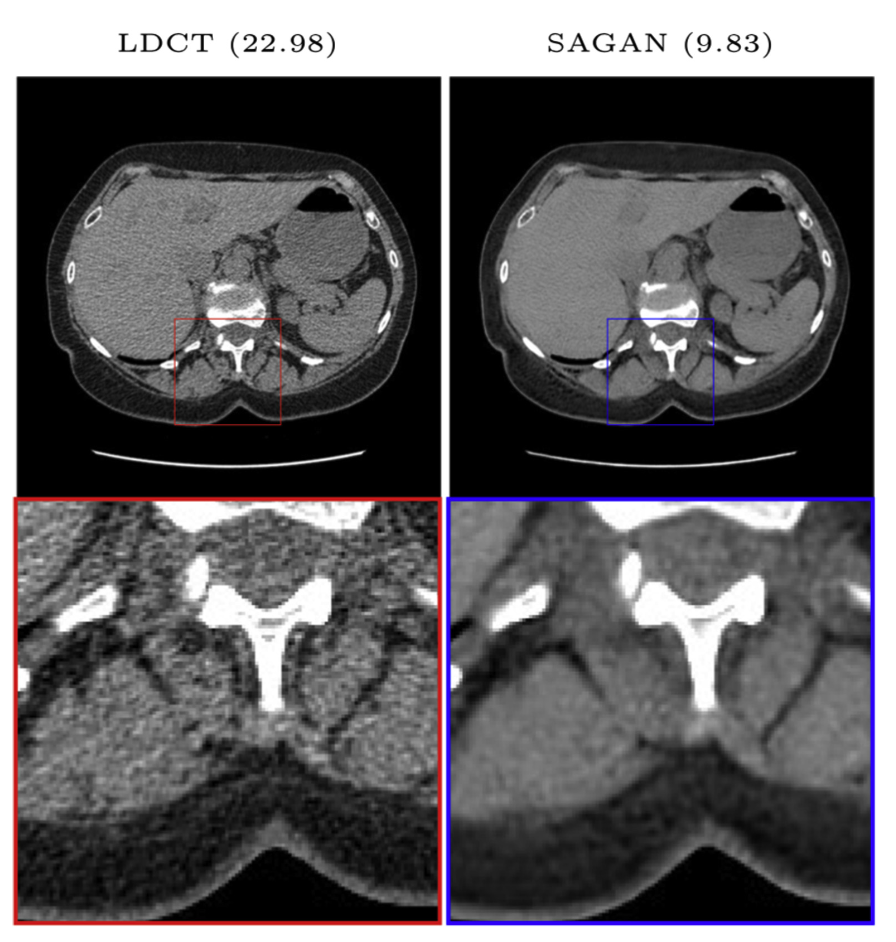
\includegraphics[width=9.5cm]{resultsVey.png}
\centering
\caption{Low Dose CT image improvement with SAGAN result}
\end{figure}

Beyond CT, GANs have been applied to generate MR and PET scans, too, with the majority focusing on either simulating rare disease scenarios or augmenting datasets.[9, 58, 59] Such synthetic data helps to improve the robustness of machine learning models for medical applications and allows AI-based diagnostic tools to operate across a larger range of patients.

Vey et al. (2019) underscore the importance of medical imaging diagnostic processes and automation using GANs, reflecting on the potential these techniques have to change diagnostic imaging approaches. In the study published in the Journal of the American College of Radiology, the authors describe the effectiveness of GANs in producing synthetic low-dose CT images, which greatly minimizes radiation risk when compared to conventional imaging processes. Furthermore, the authors articulated how highly realistic images are produced by GANs through learning from high-resolution datasets, which enables robust clinical diagnostics and AI model training.

Moreover, Vey et al. highlighted the use of GANs for the creation of synthetic low-dose CT images, pointing out their ability to solve other adversary challenges such as image artifacts that obstruct normal CT diagnostic processes. The authors believe that these findings demonstrate that the image quality of low-dose scans generated with the use of GANs can be heightened to the degree that critical elements of an examination are accessible without overexposing the patient. 

The article also stressed the effectiveness of GANs in creating synthetic data for uncommon diseases and weaving algorithms that are able to recognize a vast array of pathological processes. All in all, this represents a tremendous step, with their research being extremely influential in the intelligent diagnosis and treatment of cancer.


\subsection{High-Resolution Image Generation}

High metaphor medical images are vital to exact diagnostics, as they deliver the details wanted to pick unlikely abnormalities and differences. Nonetheless, capturing these high-resolution images is limited by technology, risk of radiation exposure, or is simply too expensive. Generative Adversarial Networks or GANs have shown great promise in solving these problems by generating high-resolution medical images from lower-resolution image.

Du and Tian \cite{Du2024} recently employed a GAN architecture with a combination of super-resolution medical images to Transformer networks. This approach exploits GANs for naturalistic image synthesis and the capability of the Transformer to recognize complex structural processes in the data. Using these models for medical imaging has allowed researchers to reach more clearer and detailed images, turning low-resolution images into high-resolution images, and ultimately providing its promises for better diagnosis.

Generative adversarial network (GAN) models operating with high resolutions have had an influence on radiology and pathology, where one detail can be critical for a correct diagnosis. In particular, GANs enhance the qualities of blurry or pixelated images from low-dose CT scans, allowing clinicians to evaluate and diagnose cancers more confidently while increasing the radiation dose [14]. Furthermore, in histopathology, where tissue images containing details of cells are necessary for specificity, higher-resolution-GANs can provide clearer and more discernable images to identify specifically cancerous or other atypical cells.

Generative Adversarial Networks (GAN) generate high-resolution versions of critical scans to produce more precise and diagnostic effective diagnoses with a reduced requirement for high-dose imaging or expensive upgrade of equipment. Not only does this feature emphasize protecting patient safety, but it also expands access to high-quality imaging in low-resource environments.

\section{Applications of GANs in Medical Imaging}
\subsection{Lung Imaging and Reconstruction}

Lung imaging is critical for the diagnosis of lung cancer and pulmonary diseases and needs high-resolution scans to obtain and visualise high-detail anatomical structures and enhance lesions. Nevertheless, low radiation protocols or the limitations of the imaging instrument can also produce images of suboptimal quality, which may ultimately compromise the diagnostic process. This has resulted in the introduction of generative adversarial networks (GANs) as a powerful technique for lung image enhancement and reconstruction, allowing for lung image resolution and clarity improvements without subjecting patients to additional radiation exposure.

In their study, Hsieh et al. Using GANs to generate high-resolution computed tomographic (CT) images of the lungs was demonstrated by \cite{Hsieh2020}. Using the GAN (generative adversarial network) model, they were able to train their models on various high-resolution lung CT datasets and reconstruct similar lung images by converting lower-resolution images to the desired outputs (high similarity outputs between input→output by improving quality). This represents a significant milestone, particularly in the reduction of radiation to patients requiring scans at frequent intervals, where images need to be diagnostically relevant but still require high exposures.

\begin{figure}[h]
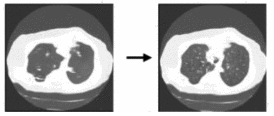
\includegraphics[]{resultsLung.png}
\centering
\caption{Lung CT reconstruction results}
\end{figure}

Usage of GANs in lung image reconstruction would not only increase its resolution but also tackle common artefacts and noise in CT imaging. This leads to cleaner images from the GAN which helps in the segmentation and accurate analysis of lung structures by removing or minimising element. This attribute is essential to detect early signs of diseases, including tiny nodules or small changes in lung tissue that might signify the development of diseases such as lung cancer or chronic obstructive pulmonary disease (COPD).


In addition, GANs do not only improve resolution but also solve various common CT imaging problems including artifacts and noise. With the noise removed, the pictures that result from the GAN model have greater clarity and therefore allow for more accurate segmentation and classification of lung structures. This capability helps in spotting the subtle early biomarkers of diseases, such as scant nodules and slight changes in tissues that are usually the first signs of lung cancer or chronic obstructive pulmonary disease (COPD). By improving the quality of these landmark features, GANs facilitate disease monitoring and enhance the sensitivity of the detection system.

Besides resolution correction, GANs can assist in image creation and augmentation which is necessary for the development of deep learning models in diagnostic AI tools. Having the ability to produce realistic synthetic lung CT images, GANs help to diversify the datasets, especially for scarce conditions, hence improving the performance of the AI-based diagnostic models.

In summary, GAN-based lung imaging and reconstruction streamlines the diagnostic process and enhances patient safety. It gives clinicians better imaging capabilities that are non-invasive and do not require a high-dose scan. Such technology could support early detection and treatment planning in respiratory care, especially in settings that have limited access to quality imaging resources.

\subsection{Brain and Heart Volumetric Data Synthesis}
Volumetric imaging is essential for the diagnosis and follow-up of complex diseases, particularly in organs such as the brain and heart. Conventional 3D imaging techniques like MRI and CT scans provide precise, high-resolution cross-sectional image data but require considerable resources, often in the theatre, and involve radiation exposure to the patient. In recent times, GANs have proposed an efficient way to alleviate this problem by generating realistic synthetic 3D volumetric data and benefiting from the augmentation of real imaging datasets to improve the training of diagnostic algorithms.

Liu et al. \cite{Liu2024} published a detailed review on GAN applications in 3D brain and heart imaging that also highlighted how GANs can also synthesize realistic volumetric data. GAN models learn from real-world 3D scans to generate synthetic but anatomically correct 3D models, providing data for 3D machine learning-based medical data modelling and testing. As an example, GANs generated synthetic brain volumes that can be used in studying neurodegenerative diseases such as Alzheimer's and Parkinson's with a dataset with numerous samples representing various stages and patterns of disease evolution.

Generative Adversarial Networks (GANs) have recently found utility in cardiac imaging by generating 3D heart models with realistic detailed structural and functional characteristics. The development will assist in the diagnosis of conditions such as cardiomyopathy and heart failure. These synthetic hearts could improve conventional diagnostic tools reliant on 3D data for accurate segmentation, classification, and analysis of cardiac components. In addition, the data generated via GANs enhances existing training datasets for deep learning models and enables them to generalize across multiple heart diseases without the need for an extensive real data collection process.

GANs contribute significantly towards the research and clinical applications for the synthesis of volumetric data for the brain and heart. GANs help researchers and clinicians by providing enhanced datasets by augmenting the existing 3D data, increasing the robustness of the AI diagnostic system. Additionally, GANs also enable research of rare diseases by generating synthetic instances of otherwise hard-to-acquire cases, thereby enhancing the effectiveness and accuracy of medical imaging technologies in the fields of both neurology and cardiology.

From aiding in diagnostics to advanced surgical planning and medicine tailoring, the applicability of generative adversarial neural networks (GANs) knows no bounds. Suited for virtual simulations of surgical interventions or other treatment protocols, GANs synthesize 3D customization specific to individual patients from minimal imaging data. For example, an electrophysiological simulation of catheter ablation on the arrhythmic heart can be performed on a 3D heart model generated by GAN as a computer-aided design. Synthetic models of the brain are useful in formulating approaches for neurosurgical tumour or vascular malformation surgeries. 

In conclusion, the GAN approach to volumetric imaging is undoubtedly a paradigm shift in medical imaging and research. The ability of GANs to produce high-grade synthetic datasets, increase image quality, and support anatomic modelling allows plugging significant gaps in conventional imaging technology. These strides are bound to benefit a patient population struggling with the challenge of timely intervention in multifaceted disorders of the nervous and cardiovascular systems. The development of the generative adversarial networks will make transitions into clinical routines of the radiology department easier, and as a result, enhance imaging efficiency and cost-effectiveness, and availability of proper diagnostic aids. These factors will significantly improve healthcare quality as a whole.



\section{GANs for Data Enhancement in Diagnostic Applications}
\subsection{Speech and Writing Analysis in Parkinson’s Disease}
Parkinson's disease (PD) is a degenerative, long-term neurological disease that affects movement and may also cause complications with speech and writing. Objective: Accurate and timely diagnosis of PD is critical for effective treatment; however, traditional diagnostic methods are invasive, expensive, and typically based on subjective assessments. Generating adversarial network GANs have recently emerged as a promising tool for speech and handwriting analysis, providing a non-invasive and inexpensive method for the diagnosis of PD — an important step towards the effective treatment of the disease.

In their study, Ilesan et al. Applying GANs to find patterns in speech and writing with potential association to PD has been explored by \cite{Ilesan2024} Guided by existing data of patients with PD, GAN models can generate synthetic samples approaching the nuances of motor challenges associated with the condition. This synthetic data enables researchers to augment datasets used to train diagnostic algorithms, covering a wider spectrum of symptom expressions through diverse stages of the disease.

In cases where GANs are utilized, they are used to increase the accuracy of feature extraction from both speech and writing focusing on traits such as voice tremor, handwriting speed, and letter formation. GANs can amplify subtle changes in speech patterns—such as changes in voice pitch, tone, and cadence—that may be difficult for clinicians to detect without expensive machines, for instance. GANs have proven useful in handwriting analysis — identifying stroke patterns and pressure irregularities that indicate early indicators of motor decline associated with the onset of Parkinsons' disease.

There are several advantages to using GANs for the analysis of speech and writing when it comes to diagnosing Parkinson's. By creating and assessing synthetic data, GANs help to lower the dependency on large sets of actual patient data—which can be difficult to procure. They may also help create more complex models that can identify PD-specific characteristics across patient populations. This can, in the future, enable the identification of tools to provide easier and larger-scale diagnostics that can assist clinicians with the early diagnosis and long-term assessment of PD.

\subsection{Artifact Correction and Noise Reduction}

Artifacts in medical imaging such as noise can significantly impact image quality, making it difficult for clinicians to read a scan correctly. Known causes of these issues include the motion of the patient, limitations of the equipment, or low-dose imaging protocols used to decrease the radiation dose to the patient. Generative Adversarial Networks (GANs) can, by reducing noise, correct these artefacts and generate clearer, high-quality images that give a higher accuracy of diagnostic.

Vey et al. Two approaches to the application of GANs in medicine are most frequent, \cite{Vey2019}: (i) enhancing quality of medical images with resolution and quality of obtained images (reducing noise, improving image quality) especially in MRI and CT scans by removing artefacts and (ii) improving images obtained from imaging methods. GANs are trained on paired datasets of high- and low-quality images and learn how to transform a noisy, artifact image into a clear image. In generating a "denoised" or "correct" image, while the discriminator checks that the output is similar to ground truth and high-quality images x, gradually correcting the generator doing this it only "polishes" at the end.

Low-dose CT imaging is another common and useful application of GANs to artefact correction, as it can produce grainy, low-quality scans due to decreased radiation. With GANs, radiologists can see the detail of a standard-dose image without additional radiation exposure to the patient. Similarly, GANs have also been used for artifact reduction in MRI scans, such as in reducing artefacts from patient movement or equipment noise that can both mask important diagnostic features.

\begin{figure}[h]
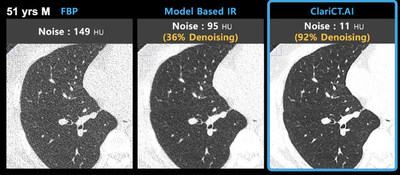
\includegraphics[height=5.5cm]{exemplificationOfNoise.jpg}
\centering
\caption{Example of noise reduction on CT Image \cite{ClariPi2021}}
\end{figure}

GAN-based artifact correction and noise reduction have been known great significant in improving the quality of medical practicable images without invasion and with economic expenses. Not only does this approach help improve diagnosis and treatment planning but it also allows high-quality imaging to be more accessible in resource-constrained environments by enabling lower dose and less expensive imaging solutions.

\section{Challenges and Future Directions}

While GANs have the potential to revolutionize medical imaging and diagnostics, there are still several hurdles to overcome before they can be fully integrated into clinical practice. These hurdles encompass technical limitations, concerns about data privacy, regulatory issues, and the necessity for additional research to improve the robustness and interpretability of the models.

\subsection{Technical Limitations}

Training GANs can be quite unstable and often requires significant computational resources. To achieve high-quality results, it's essential to carefully adjust model parameters and address challenges like mode collapse, where the generator ends up producing a narrow range of outputs instead of reflecting the full diversity of the data. Moreover, GANs are very sensitive to both the quality and quantity of training data, which can be particularly challenging to gather in medical fields due to privacy concerns and limited data availability.

\subsection{Ethical concerns}

Medical data is extremely sensitive, and utilizing it to train GANs brings up significant concerns regarding patient privacy and data security. Although generating synthetic data can help alleviate these issues by minimizing the reliance on actual patient data, it is crucial to ensure that synthetic data does not unintentionally contain identifiable information. Tackling these privacy issues is vital for the ethical application of GANs in healthcare, particularly in areas with stringent data protection laws such as GDPR in the European Union.

\subsection{Regulatory and Standardization Barriers}

Validation of safety and effectiveness is critical before any GAN-generated images are incorporated into the clinical workflow. Stipulations by the FDA and EMA do not yet exist for the approval of synthetic medical images for diagnostic purposes, nor is there a standard for the use of such devices.

\subsection{Interpretability and Trustworthiness of Models}

Since GANs operate as a black box, this limits their clinical application because healthcare workers might not be willing to rely on diagnostic procedures that lack proper reasoning. Adding model explainability to synthetic image generation and assessment by employing attention maps, saliency maps, or other model-agnostic explanations can augment clinician understanding. In order to integrate and trust clinical decision making aids generated by GANs, clinicians need to be provided trustworthy visualizations and explanations of the GAN outputs.

\subsection{Need for Extensive Clinical Validation and Longitudinal Studies}

In addition, the acceptance of GANs into clinical practice will require large-scale multi-institution studies with different patient populations and imaging modalities to validate the effectiveness of the system. Furthermore, studies that measure the patient’s clinical outcome over time in relation to the use of GAN-based diagnosticians will be needed to determine the long term prognosis of this type of clinical care. Collaborations between researchers, clinicians, and governing bodies are vital in the design and conduct of these studies.

\subsection{Future Directions}
To address these challenges, future research in GANs for medical applications could focus on several key areas:

\begin{enumerate}
    
\item Hybrid Models: Combining GANs with other architectures, such as transformers or variational autoencoders, may improve stability and allow for more efficient training, leading to higher-quality outputs.
\item Privacy-Preserving Techniques: Integrating techniques like federated learning or differential privacy can help safeguard patient data during GAN training, allowing models to learn from distributed datasets without centralizing sensitive information.
\item Improved Evaluation Metrics: Developing metrics tailored to assess the clinical relevance and accuracy of GAN-generated images would facilitate objective model evaluation and enhance clinical acceptance.
\item Real-World Implementation Studies: Collaborations between AI researchers, clinicians, and regulatory bodies can help bridge the gap between research and practice, providing insights into the real-world impact, challenges, and requirements for GAN deployment in clinical settings.
\end{enumerate}

\section{Implementation of methods}

\subsection{Generating Parkinson's Disease Gait Patterns \cite{Ilesan2024}}

Training a Generative Adversarial Network (GAN) can be challenging, involving temporary setbacks and issues that need to be overcome to achieve a good result. For this implementation, the chosen dataset contains gait correlation matrices that belong to healthy people and patients who were diagnosed with Parkinson's disease and the goal is to create a model and train it to reproduce Parkinson's Disease gait patterns in new images that can be used in the future training of a possible classification model or translated into real movements that can help doctors find new patterns of movement that led to early diagnosis.

The training progress of the GAN model can be observed through the outputs generated at different epochs. These outputs provide valuable insights into the model's learning and development.

\begin{figure}[h]
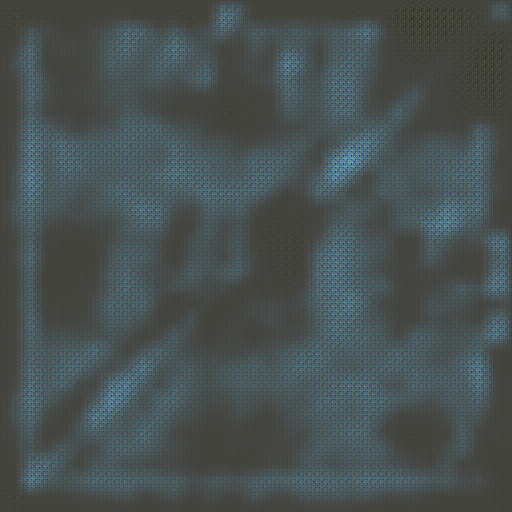
\includegraphics[width=5 cm]{generated50.png}
\centering
\caption{50th Epoch Output}
\end{figure}

As shown in the previous figure, the output of the 50th training epoch demonstrates that the generator model has successfully identified and contoured the areas of interest within the generated image. This includes the left and right plantar pressure progression, as well as the tremor. This is a positive indication that the models are learning effectively and progressing along a favourable path.
\newpage

\begin{figure}[h]
    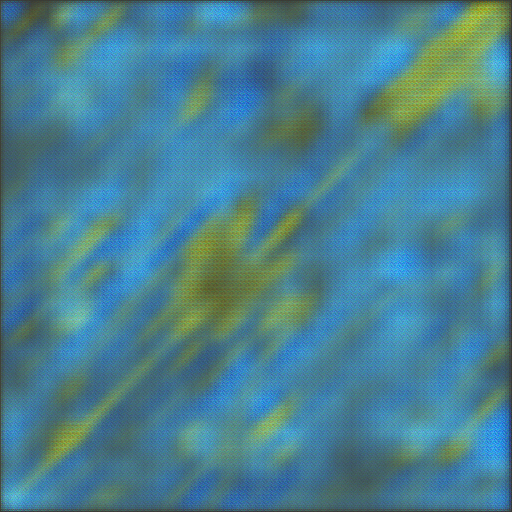
\includegraphics[width=5 cm]{generated150.png}
    \centering
    \caption{140th Epoch Output}
\end{figure}

As the training continued to the 140th epoch, the generator model exhibited a significant advancement in its capabilities. Not only did it accurately highlight the areas of interest, but it also began to illustrate the correlation colors in the generated images. This resulted in a more realistic representation of the correlation matrix.

\begin{figure}[h]
\centering

\includegraphics[width=5cm]{generated350.png}
\caption{350th Epoch Output}
\end{figure}


The GAN model's training progressed beyond the 350th epoch, and we observed persistent improvements in the quality of the generated correlation matrices. As the training advanced, the contours and illustrations of the small correlation matrices became more evident, showcasing the generator model's increased ability to capture complex details and accurately reproduce the physiological patterns of gait. 


\begin{figure}[h]
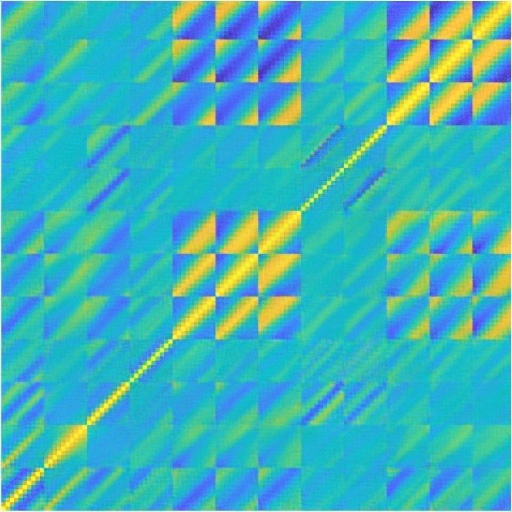
\includegraphics[width=5 cm]{generated_img_24000_0.png}
\centering
\caption{24000th Epoch Output}
\end{figure}


In the 24000th epoch, the output quality was considerably good with images that successfully reproduced Parkinson's Disease patterns. 

After an extensive training process spanning 40000 epochs, the generated correlation matrices generated were very similar to the real ones. The generated images were almost indistinguishable from the real ones. 

\begin{figure}[h]
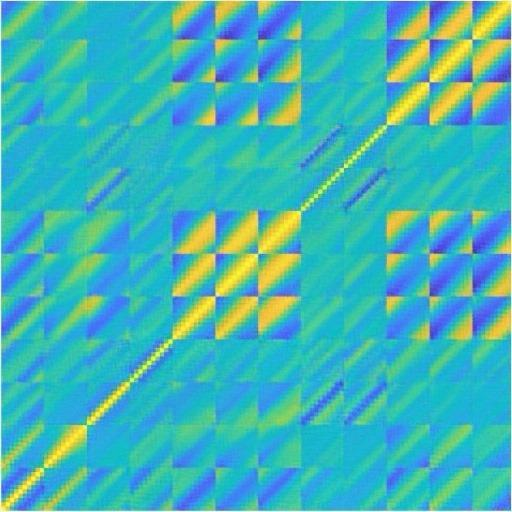
\includegraphics[width=5 cm]{generated40000.jpeg}
\centering
\caption{40000th Epoch Output}
\end{figure}

The output of the generator model shows a notable noise reduction, contributing to a clear illustration of the correlation matrices. Additionally, the accurate color representation in the generated matrices validates that the generator model has effectively learned to generate the images in a proper and realistic manner.

These remarkable results outmatch the initial expectations and demonstrate the potential of the GAN approach in generating high-quality synthetic data that can augment and support
research efforts in understanding Parkinson’s disease and other movement disorders.

\subsection{Generating Lung CT Tumor Images}
This implementation employs a Generative Adversarial Network to synthesise lung CT images sliced from Chest CTs containing tumor patterns. The dataset consists of CT scans from patients with diagnosed lung tumors and healthy controls. The goal here is to implement a GAN model to generate realistic tumor-affected CTs, which will help build a new dataset for tumor segmentation.

The training progress of the GAN model performed similarly to the first implementation. The model was able to replicate tumors find tumors in the images and learn different tumor types and replicate them.

\begin{figure}[h]
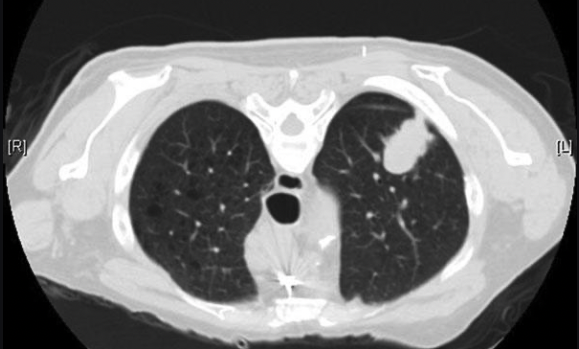
\includegraphics[width=9cm]{tumorReplicated.png}
\centering
\caption{Example of a lung tumor in big perspective}
\end{figure}

In the training process the model was able to reproduce different types of tumors that were described in the dataset very precisely. After circa 30000 epochs, the model could generate and integrate into the CT image real-like tumors.

\begin{figure}[h]
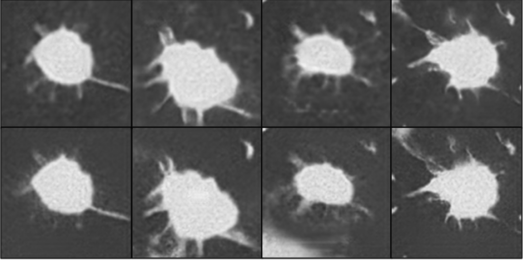
\includegraphics[width=9cm]{generatedTumorsSet1.png}
\centering
\caption{Tumors generated by the model mid-training}
\end{figure}


The results were good, but the metrics showed that the model still has potential, unlike the first implementation where the training stopped at 40000 epochs, this model was still learning and providing better images after this checkpoint.
This can be explained by the difference in the complexity of the models, the lung tumor model being more complex than the Parkinson's disease one.

After some more hours of training the model metrics reached the expectations and the training automatically stopped (EarlyStopping metric was used). 
The results were very good, the model successfully produced high-fidelity synthetic tumors demonstrating its potential for enhancing the segmentation dataset.

\begin{figure}[h]
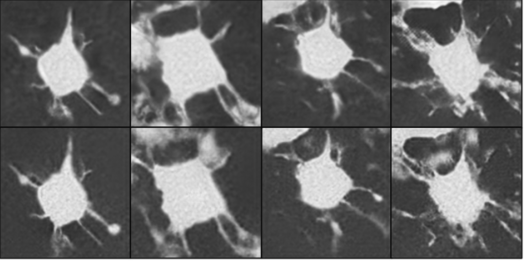
\includegraphics[width=9cm]{generatedTumorsFinal.png}
\centering
\caption{Tumors generated by the final model}
\end{figure}


\section{Implementation Conclusions}

By implementing the methods of the papers presented in this SotA article it is evident not only that the papers chose a good approach in meeting their goal, but also that they provided good value to the research by providing solutions to one of the biggest concerns in the medical field, patient early diagnosis. This concern is critical in many cases, especially in the case of cancer where time is the most important aspect in providing good treatment and hopefully curing the tumor. These findings underscore the value of GAN-generated datasets that augment training resources and contribute in generating new datasets that can be used in new scenarios where real data is not enough to provide a good clinical solution.


\section{Conclusion}

Generative Adversarial Networks (GANs) are emerging as a revolutionary tool in medical imaging and diagnostics, addressing some of the most significant challenges in the field. They can generate high-resolution images, enhance low-dose scans, synthesize 3D volumetric data, and support non-invasive diagnostic techniques, showcasing their impressive versatility and potential. By augmenting limited datasets, correcting imaging artefacts, and creating realistic synthetic data, GANs can significantly enhance the reliability of AI-driven diagnostic tools and broaden access to quality healthcare. 

Apart from using GANs for imaging, these tools can also be used to personalize medicine further by producing specific doctored data to simulate treatments and plan surgeries. Furthermore, GANs can advance telemedicine by creating realistic synthetic images necessary for a diagnosis, helping people even in remote locations receive proper medical attention. All of these would be possible through GANs serving a more comprehensive function in the healthcare system.

The amalgamation of GANs with other emerging technologies such as federated learning, blockchain for data storage, and quantum computing can further enhance their functionality. Using synthetic datasets, federated learning could facilitate collaborative model training at multiple sites while preserving patient confidentiality. Still, blockchain could support the protection and validity of datasets. There are many issues revolving around sharing data and protecting patient privacy in health care, and these could be solved with some of these solutions.

For clinical integration to happen, a cross-functional group consisting of researchers, clinicians, technology makers, and regulators have to work together to create guides to assess the quality of images produced from GANs. To be able to earn trust, it would also be important to formulate specific policies detailing the criteria for the validation of authentic medical data.

Nonetheless, for GANs to fully realize their clinical potential, several challenges need to be tackled. Concerns regarding training instability, data privacy, model interpretability, and regulatory compliance necessitate ongoing research and development. Future efforts, including hybrid model strategies, privacy-preserving training methods, improved evaluation metrics, and real-world clinical studies, will be crucial in closing the gap between research advancements and practical application.  In conclusion, GANs present a promising avenue in medicine, with the capacity to revolutionize diagnostic imaging, data augmentation, and patient care. Ongoing improvements in GAN technology, paired with careful application and validation, could integrate these tools into the healthcare system, enhancing diagnostic precision, facilitating early detection, and ultimately improving patient outcomes globally. \newpage

\bibliographystyle{plain}
\bibliography{refs}

\end{document}
